\section{Installation}

This section describes how to build Matchbox from the source distribution. There might be binary distributions provided...TODO


\subsection{Requirements}

\subsubsection{Open Computer Vision Library (OpenCV)}

The Open Source Computer Vision (OpenCV) libarary \cite{opencv_library} is a library of programming functions for real time computer vision.
It is released under a Berkeley Software Distribution (BSD)\footnote{http://opensource.org/licenses/bsd-license.php} license and thus is free for commercial or research use.
The library provides a wide range of implemented algorithms on image analyses, image data and matrix manipulation, basic and advanced image processing, object recognition and image feature extraction.

Most of Matchbox'es implementation is based on routines provided by OpenCV. 

\paragraph{Installing OpenCV}


\subsubsection{Python}

Python is a popular dynamic programming language. 
Python is used to model diverse use cases and workflows of document image quality assurance.

Modules required by Matchbox:

\begin{itemize}
	\item Numpy - Numerical Python
	\item Argparse - Parser for command-line options, arguments and sub-commands
\end{itemize}


\paragraph{Installing Python}

Python comes with most linux distributions out of the box. For Windows, 
install Python from the Python website \footnote{\url{http://www.python.org}}.
The additional libraries can also be found on the website or in the package repositories 
of the Linux distribution of your choice.


\subsubsection{CMake}


The binaries can also be built manually using cmake, as long as the OpenCV development files can be found on the system.
To build the binaries, the following commands have to be issued in the \verb+pc-qa-matchbox+directory:

\paragraph{Installing CMake}

For Windows, download cMake from the cMake website\footnote{\url{http://www.cmake.org/}} and install
it.

For Linux, cMake usually can be installed via the distribution package manager. 
E.g. for Ubuntu \verb+sudo aptitude install cmake+. 


\subsubsection{C++ Compiler}


\paragraph{Linux}

Matchbox can be built with gcc, a compiler 
that is shipped with most Linux distributions.

\paragraph{Windows}

On Windows, either Visual Studio or 
MinGW can be used to build.

\subsection{Optional Packages}

\subsubsection{Intel Threading Building Blocks Library (TBB)}

\subsection{Installation on Linux}

\subsubsection{Manual compilation}
Manual compilation should be straightforward:
Navigate to the source code directory and enter

\begin{verbatim}
mkdir build
cd build
cmake ..
make
sudo make install
\end{verbatim}

The commandline tools will then be available to you.

\subsubsection{Ubuntu}
A debian package for the installation of Matchbox on various Linux distributions is available.
It can be installed on Ubuntu from version 10.04 and up with the following commands:

\begin{verbatim}
sudo dpkg -i pc-qa-matchbox.deb
sudo apt-get -f install
\end{verbatim}

After the installation, the commandline tools \verb+extractfeatures+, \verb+train+,
\verb+compare+, \verb+FindDuplicates.py+ and \verb+CompareCollections.py+ are 
available.

\subsubsection{other Linux distributions}
The debian package has not been tested yet for other debian-like distributions.
However, it should work in theory, as long as the necesssary packages are present
in the package repositories.

\subsection{Installation on Windows}

\subsubsection{Compiling Matchbox using MS Visual Studio}

\subsubsection{Compiling Matchbox using MinGW}

An environment variable called OPENCV\_DIR, pointing to the 
directory where OpenCV was built, has to be defined. 
This can be done by right-clicking ``My Computer'', choosing 
``Properties'' and changing to the ``Advanced'' tab. After
clicking the button ``Environment variables'', an environment 
variable can be added.

As a next step, a MinGW Makefile has to be generated using CMake.
The GUI of cMake can be seen in figure \ref{fig:cmake}.
%TODO: Insert Cmake picture
\begin{figure}[htpb]
	\centering
	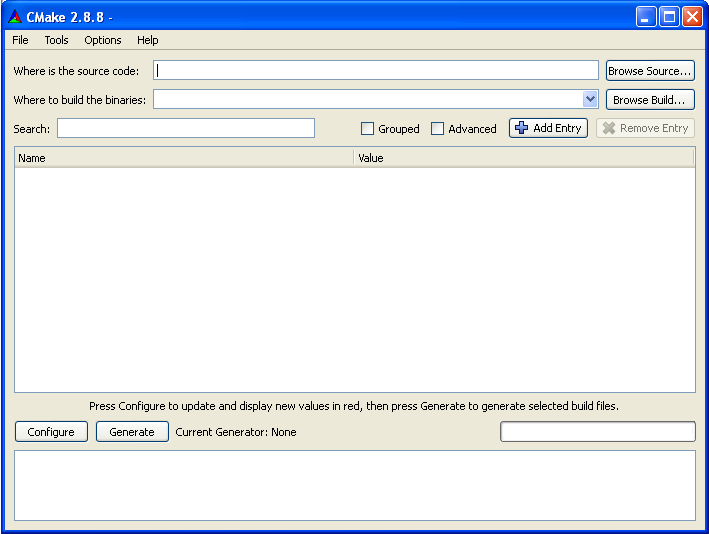
\includegraphics[width=\textwidth]{img/cmakegui}
	\caption{The graphical user interface of cMake}
	\label{fig:cmake}
\end{figure}
Start CMake, click ``Browse Source'' and find the directory containing
the Matchbox source. Click ``Browse Build'' and choose a directory
where the code will be built.
Click ``Configure'' and choose ``MinGW Makefiles'' from the dropdown menu.
Below the dropdown menu, ``Use default native compilers'' has
to be selected. Click ``Finish''. 
%TODO what can be seen after finish is clicked?
After cMake finished configuring, click
``Generate''. After cMake is done, the Makefile can be found in the
build directory.

Start the MinGW shell and navigate to the directory you specified as
build directory. Enter the command \verb+mingw32-make+ and press enter.
The sourcecode should now compile successfully.
Issuing the command \verb+mingw32-make install+ copies the executables
and libraries to the right places in the filesystem.
